\chapter{Feeding Model Terms}
\label{app:feeding-model}

Figure~\ref{fig:results-feeding-model} summarises the mixed-effects logistic model of Equation~\ref{eq:feeding-glmm} by its predicted probabilities and deficit odds ratios. The figure below shows the whole fit, including the random intercepts that summary averages over.

\begin{figure}[H]
    \centering
    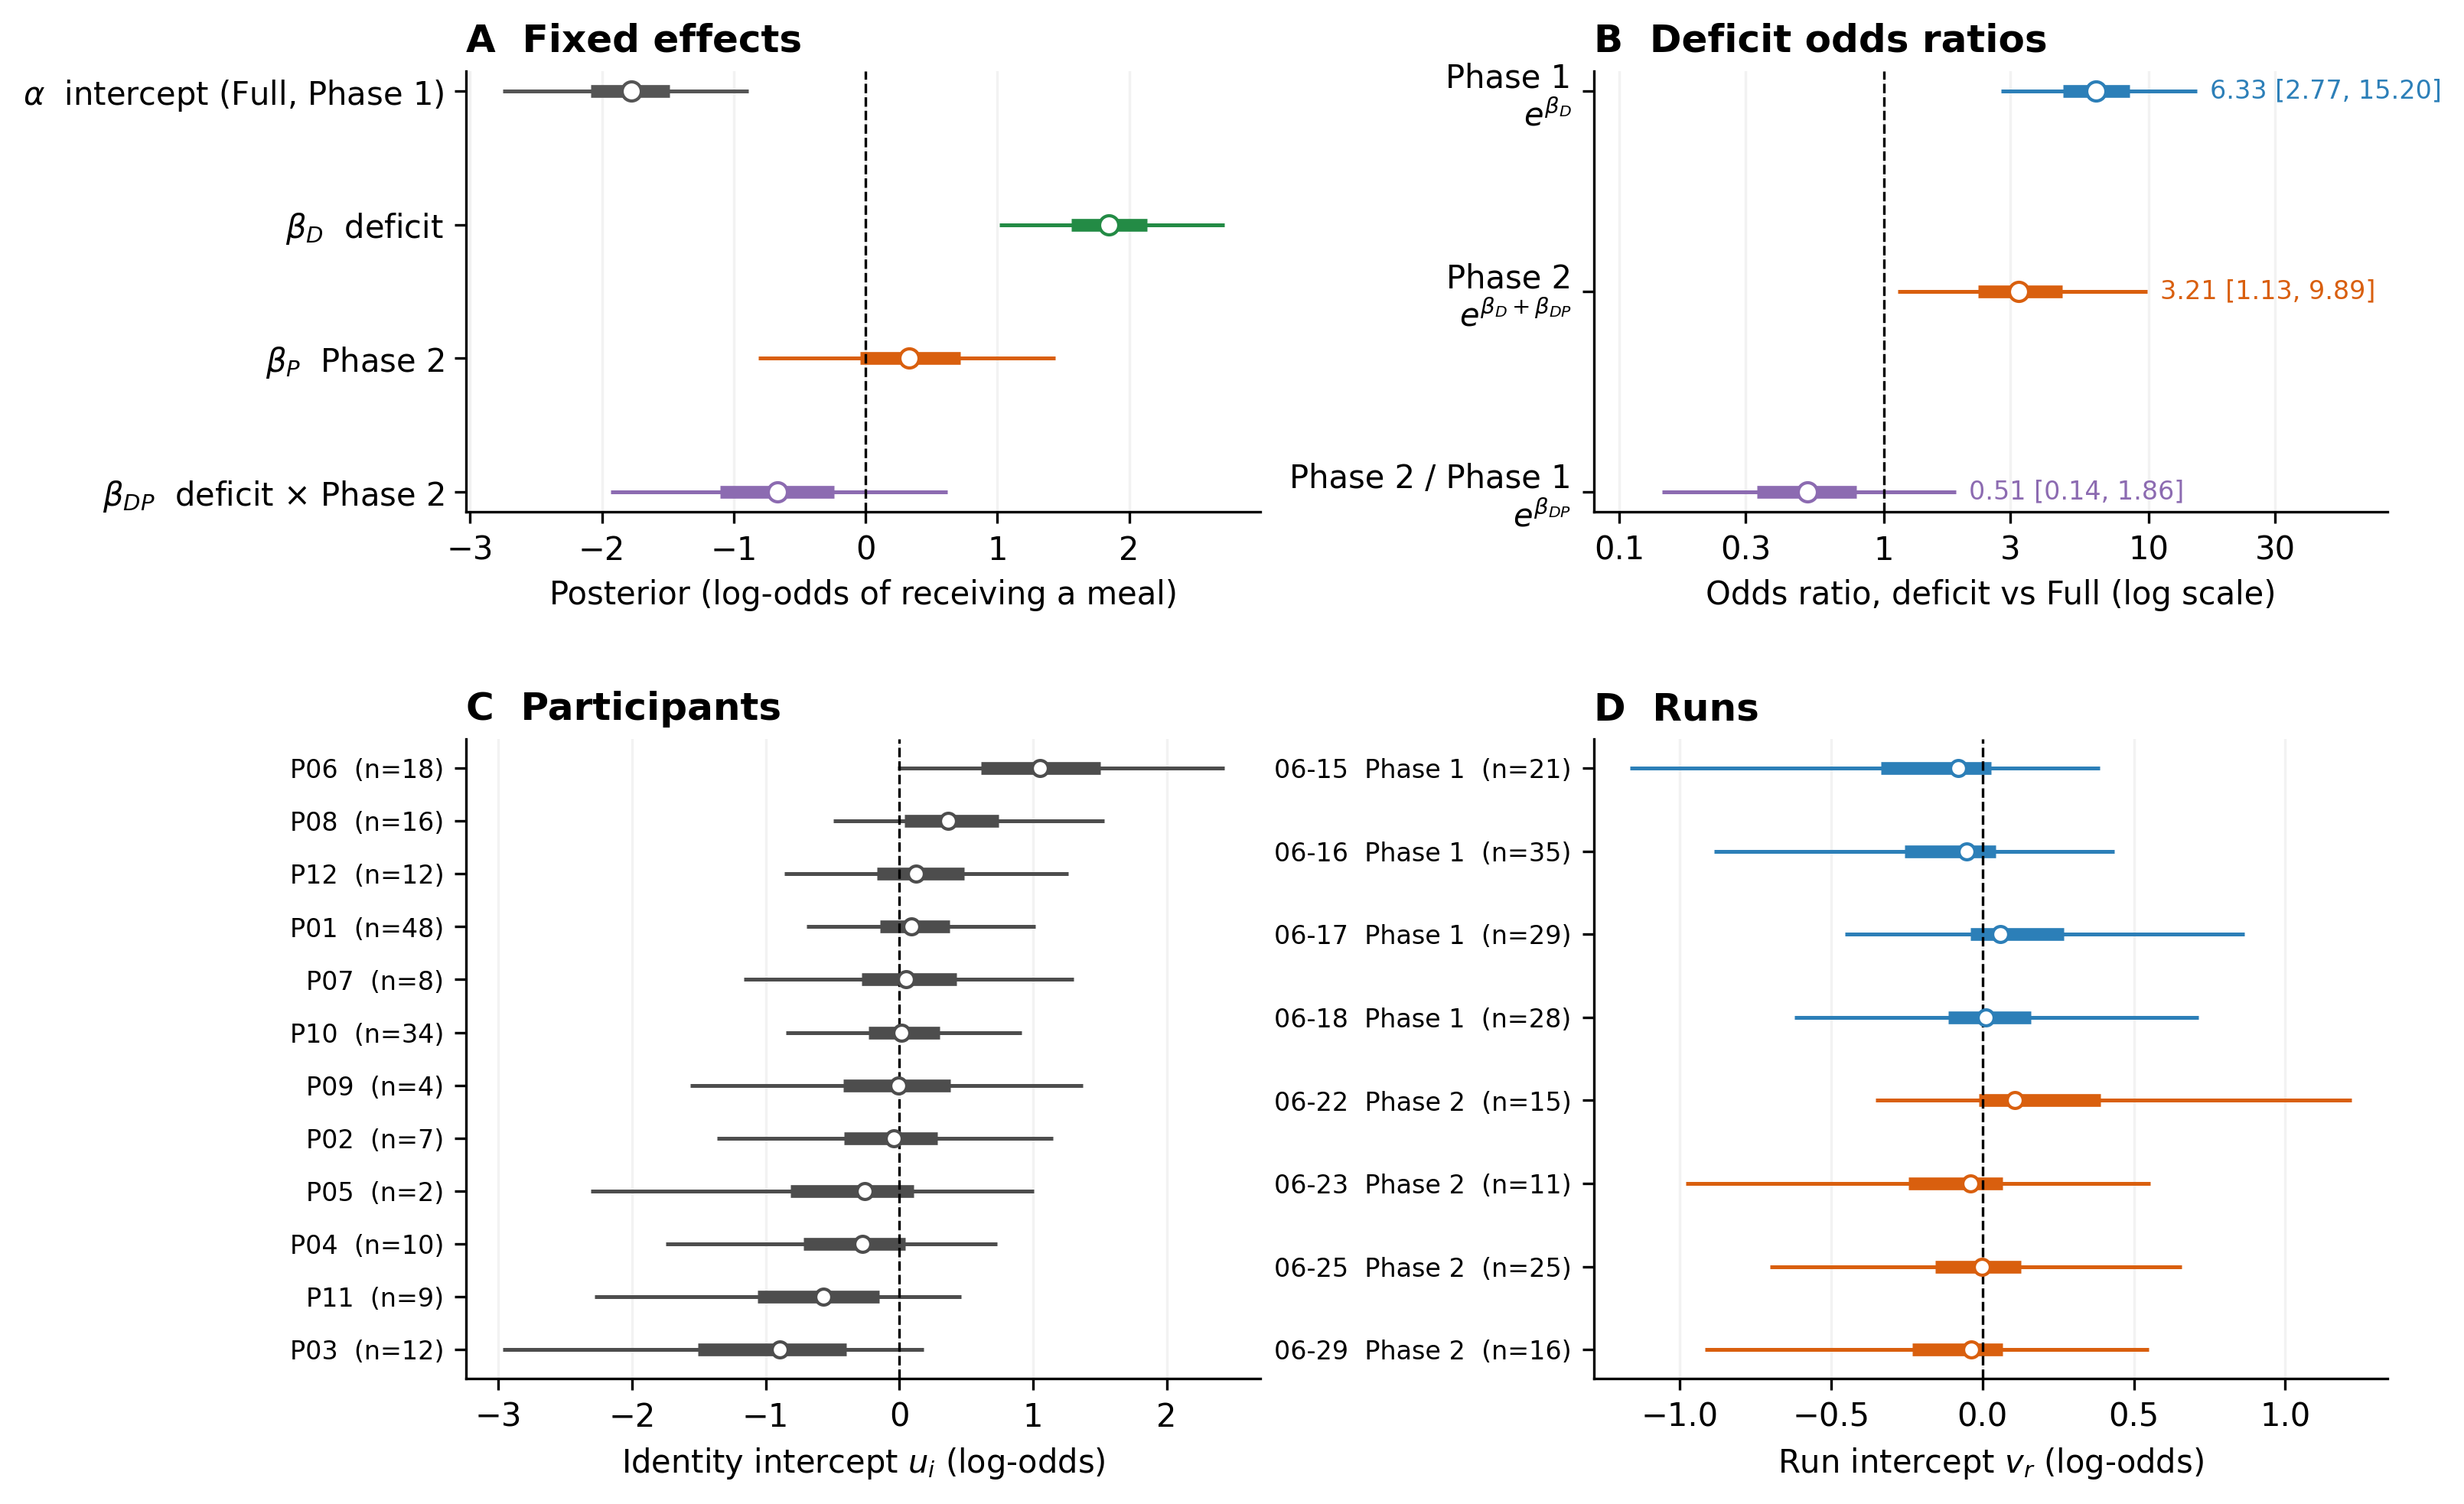
\includegraphics[width=0.8\textwidth,height=0.46\textheight,keepaspectratio]{Results/Figures/feeding-glmm-terms.png}
    \caption[Posterior terms of the feeding model.]{The fitted terms of Equation~\ref{eq:feeding-glmm}, estimated from the \CoreModelN{} named interactions. Dots are posterior medians, thick and thin bars 50\% and 95\% credible intervals, and dashed lines mark no effect. Panel A gives the fixed effects in log-odds. Panel B turns them into the deficit-to-Full odds ratios also given in Figure~\ref{fig:results-feeding-model}, together with their Phase~2-to-Phase~1 ratio. Panels C and D show how far each named identity and each deployment day departs from the average. People differed more than runs did (standard deviations \CoreModelIdentitySD{} and \CoreModelRunSD{}).}
    \label{fig:results-feeding-glmm}
\end{figure}
